%Please use LuaLaTeX or XeLaTeX
\documentclass[11pt,aspectratio=169]{beamer}
\setbeamertemplate{bibliography item}[text]
\setbeamercolor{bibliography entry author}{fg=black}
\setbeamertemplate{hyperlink symbols}{}


\title{Reinforcement Learning Based Locomotion for Variable Geometry Truss Robot }
\date[ABC 2021]{IEEE Robotics and Automation Letters}
\author{\fontsize{10}{13}\selectfont Ozgur Gulsuna}
\institute{\textbf{MMI706} \\ Reinforcement Learning}

\usetheme{eth}

\colorlet{titlefgcolor}{ETHRed}
\colorlet{accentcolor}{ETHRed}

\begin{document}

%\def\titlefigure{elements/title-page-image}		% Default image
%\def\titlefigure{elements/title-page-image-43}	    % Use this for 4:3 presentations

\def\mydate{10 Mar 2024}
\date{\mydate}

% 6 min presentation, 10 slides max

\titleframe

\tocframe

\section{Domain}

\begin{frame}[fragile]{\textbf{Variable Geometry Truss Topology}\hfill \fontsize{8}{8}\selectfont DOMAIN:ROBOTICS}
    
        \begin{textblock*}{5cm}(50mm,13mm) % {block width} (coords)
        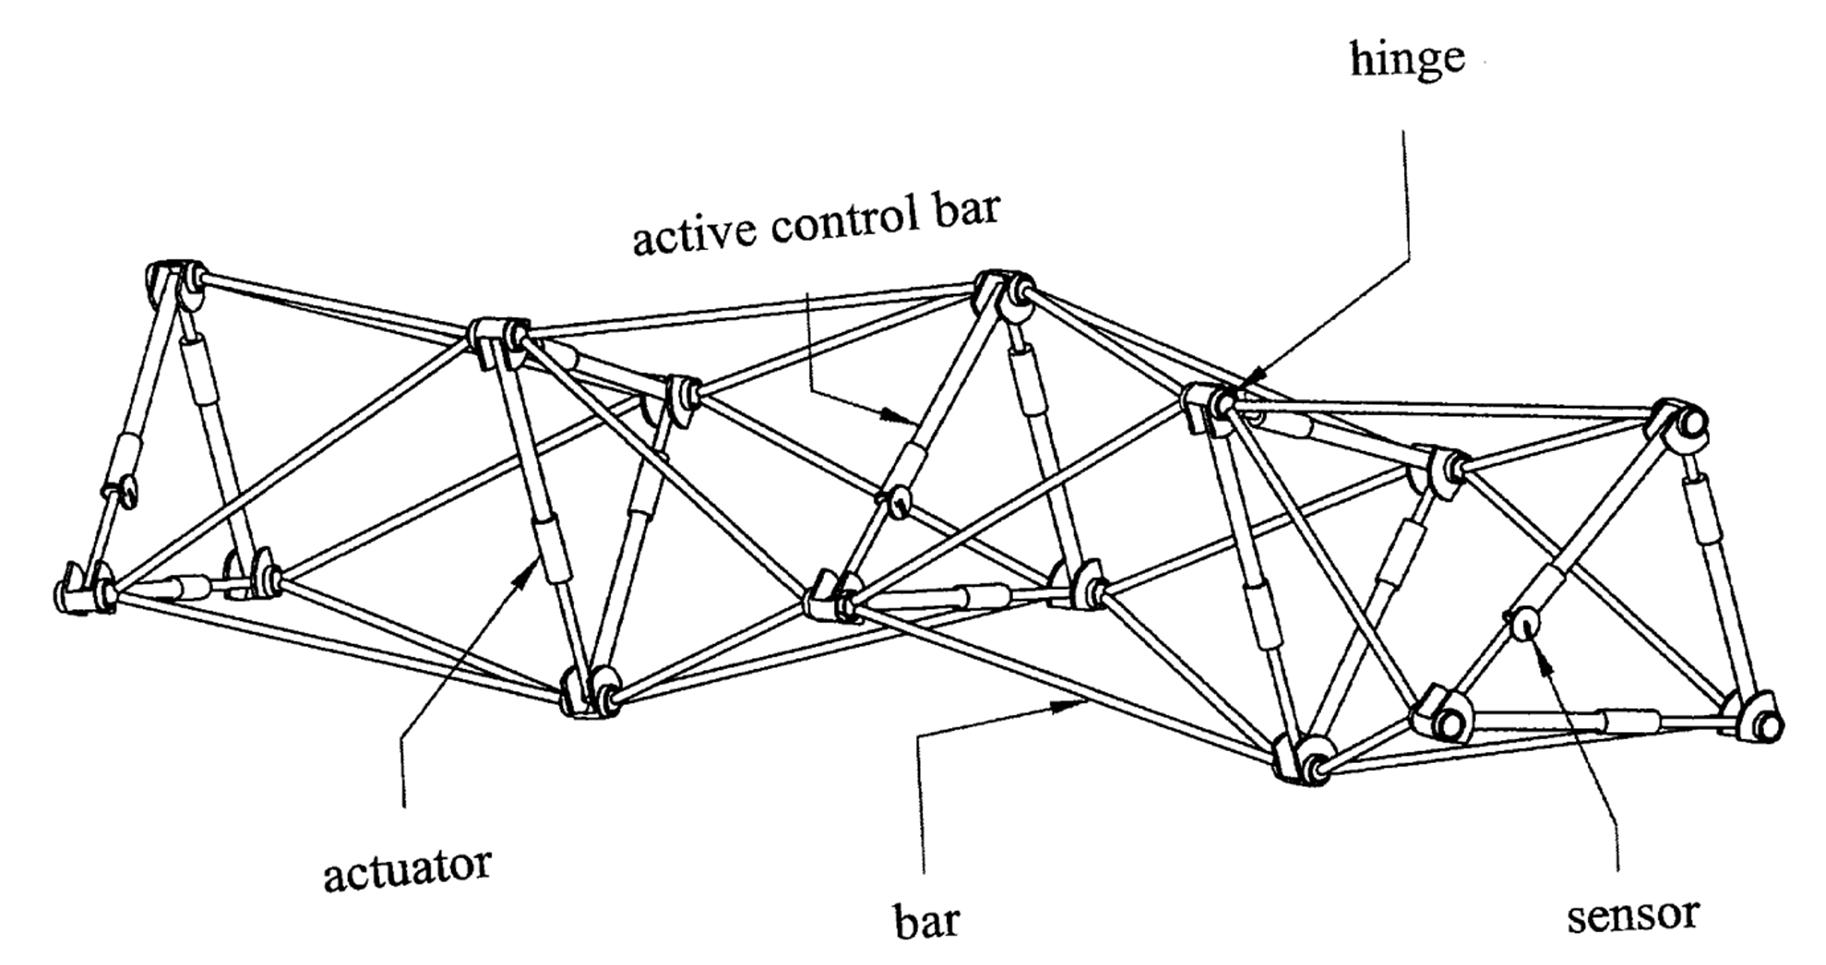
\includegraphics[height=48mm]{elements/[1]-VTT.png}
        \end{textblock*}

        Variable geometry topology (VGT) is a truss structured system that comprises actively \uline{actuated linear trusses} linked with \uline{passive rotational ball joints}.

        \medskip
        
        \begin{itemize}
            \item \textbf{Members:} Edges that are actuated linearly. \\
            has minimum and maximum lengths that are constraints.
            \item \textbf{Nodes:} Passive rotational joints. \\
            Angles between the members \\
            on joints are constrained.
        \end{itemize}

        \bigskip
        \bigskip
        \medskip
        
        \emph{Advantages:} \\
        Variable size, pass-through confined spaces.

        \medskip

        \emph{Disadvantages:} \\
        Needs a rigid actuator with high extension ratio.
 	
        \medskip

        \begin{textblock*}{5cm}(137mm,-33mm) % {block width} (coords)
        {\tiny \cite{10.1016/S0168-874X(99)00041-4}}
        \end{textblock*}
 
\end{frame}

\begin{frame}[fragile]{Realized Robots}

        \begin{textblock*}{5cm}(56mm,-30mm) % {block width} (coords)
        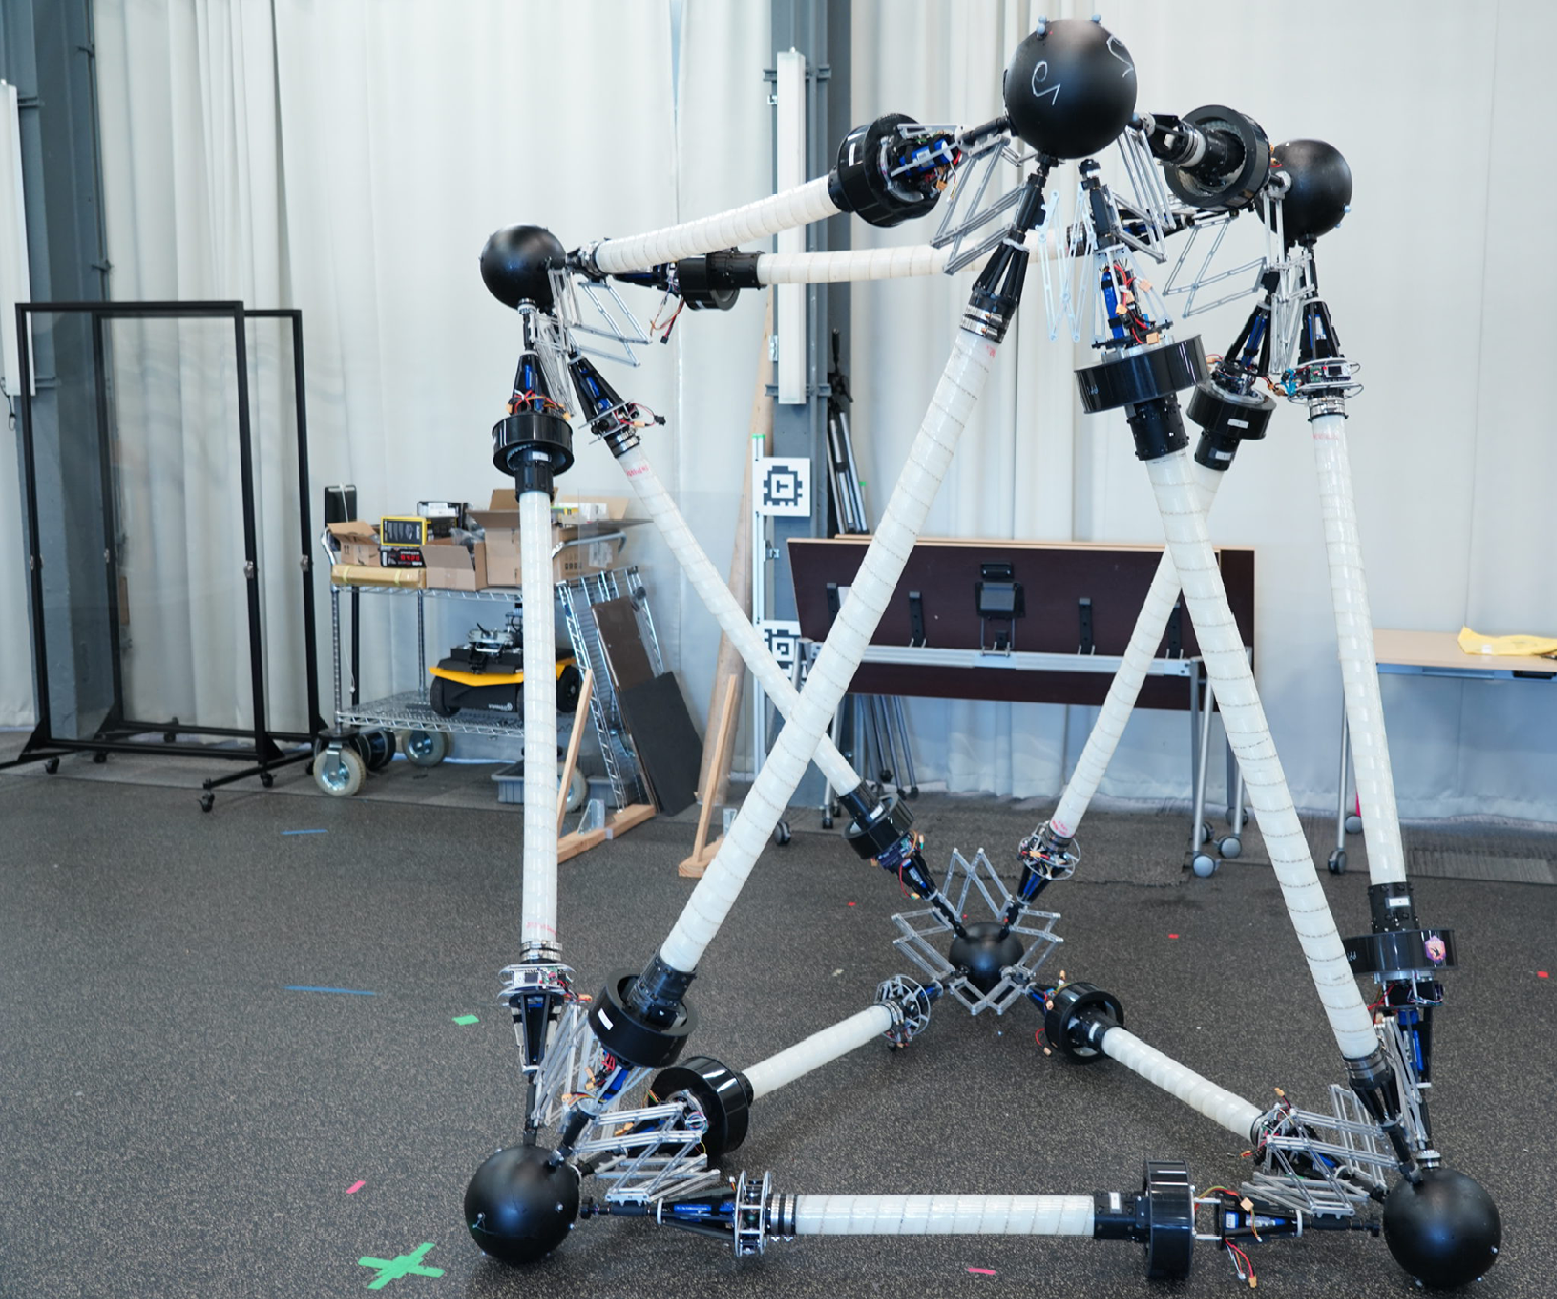
\includegraphics[height=70mm]{elements/[3]-R2.png}
        \end{textblock*}
    
        \begin{textblock*}{8cm}(0mm,-24mm) % {block width} (coords)
        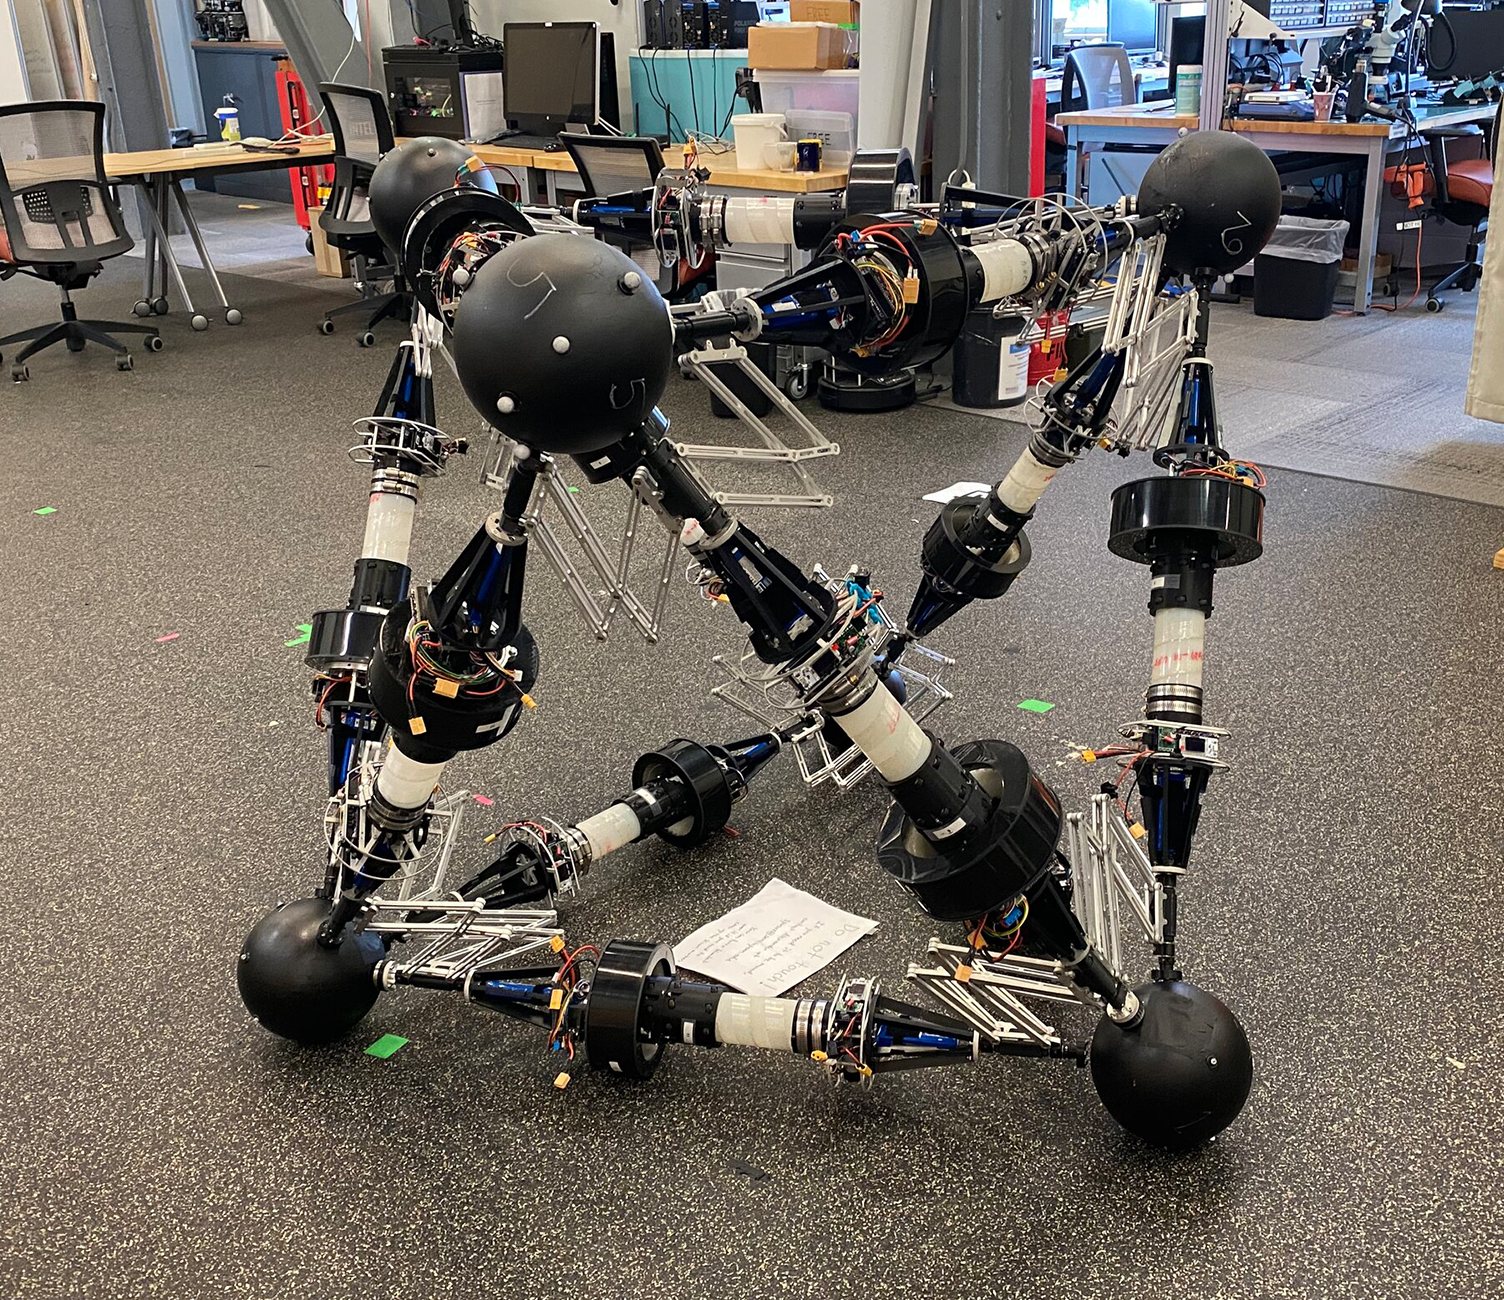
\includegraphics[height=64mm]{elements/[2]-R1.png}
        \end{textblock*}

        \begin{textblock*}{5cm}(1mm,37mm) % {block width} (coords)
        {\color{white} \tiny \cite{Guan}}
        \end{textblock*}

        \begin{textblock*}{5cm}(136.5mm,37mm) % {block width} (coords)
        {\color{white} \tiny \cite{extended}}
        \end{textblock*}
 
\end{frame}

\begin{frame}[fragile]{Realized Robots}

        \begin{textblock*}{8cm}(75mm,14mm) % {block width} (coords)
        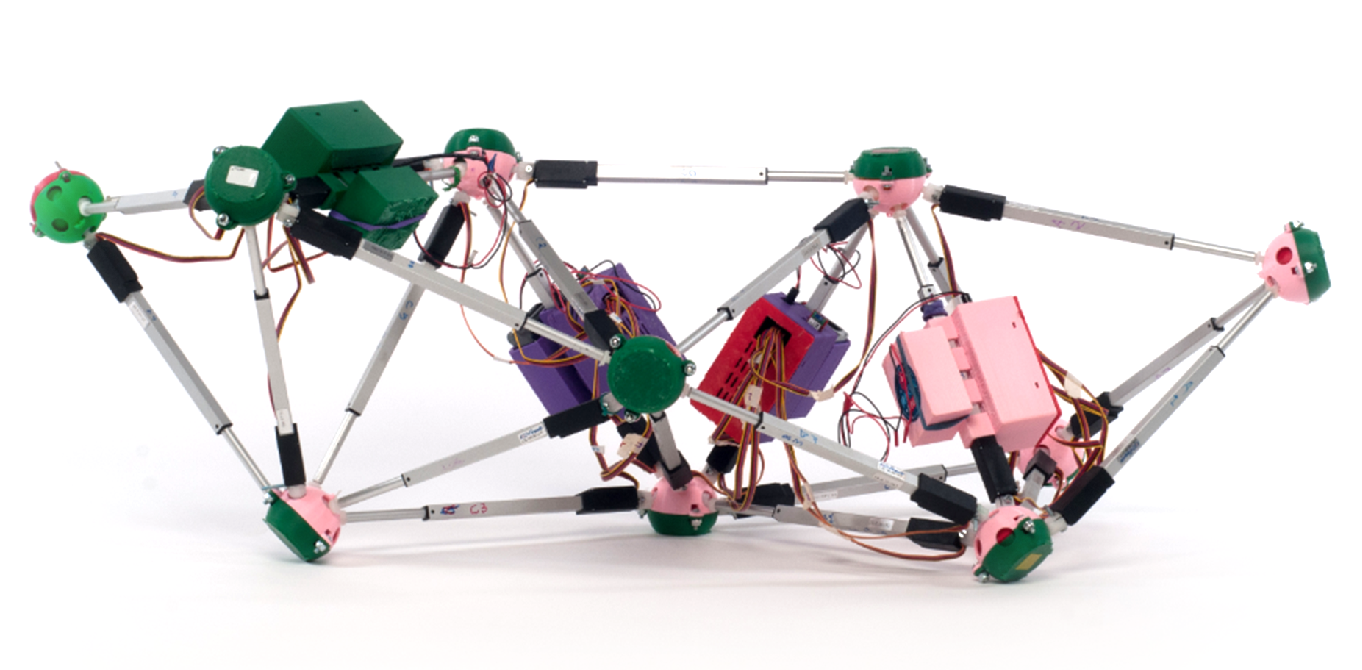
\includegraphics[height=31mm]{elements/[6]-R5.png}
        \end{textblock*} 
        
        \begin{textblock*}{8cm}(60mm,-30mm) % {block width} (coords)
        {\color{white}\href{https://youtu.be/1dMpeTp2ZrM}{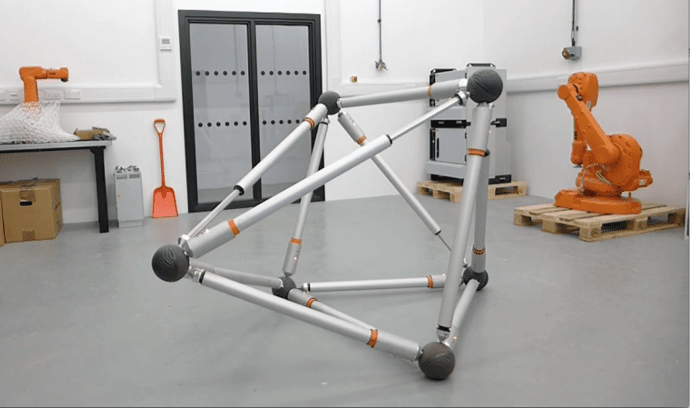
\includegraphics[height=46mm]{elements/[5]-R4.png}}}
        \end{textblock*}
    
        \begin{textblock*}{5cm}(0mm,-24mm) % {block width} (coords)
        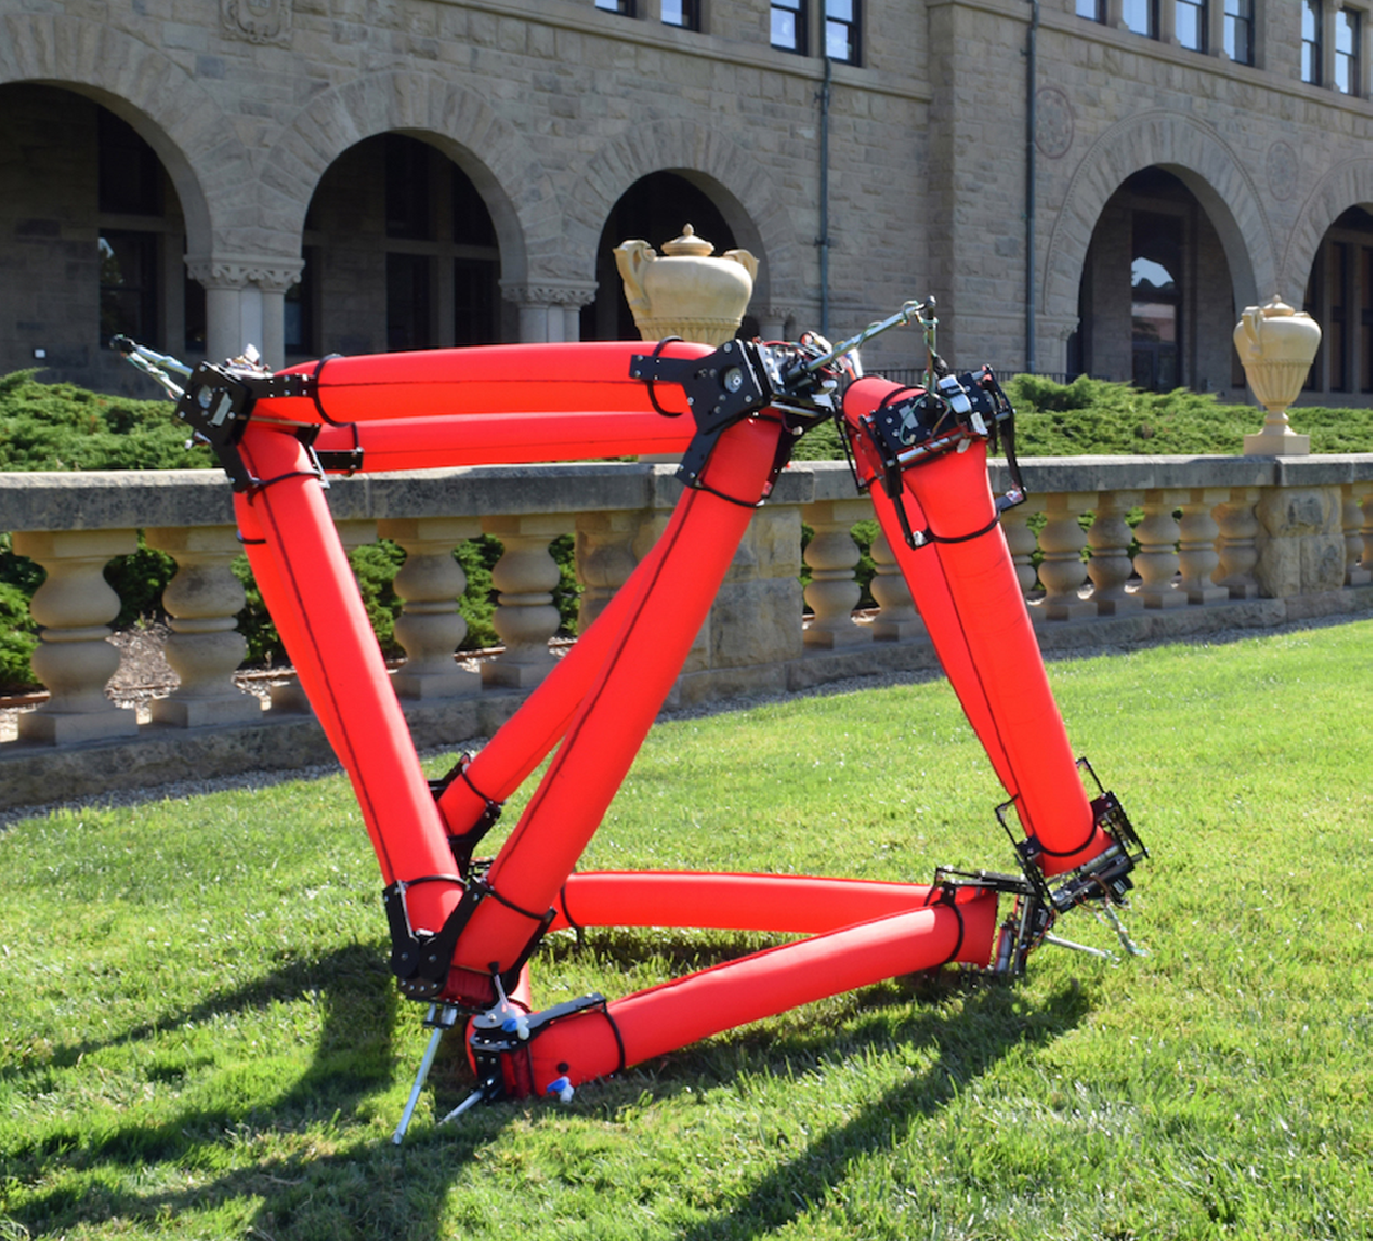
\includegraphics[height=64mm]{elements/[4]-R3.png}
        \end{textblock*}

        \begin{textblock*}{5cm}(1mm,37mm) % {block width} (coords)
        {\color{white} \tiny \cite{SHAPE}}
        \end{textblock*}

        \begin{textblock*}{5cm}(134.5mm,13mm) % {block width} (coords)
        {\color{white} \tiny \cite{william-bondin}}
        \end{textblock*}

        \begin{textblock*}{5cm}(134.5mm,38mm) % {block width} (coords)
        {\color{black} \tiny \cite{10.1145/3448326.3448332}}
        \end{textblock*}
 
\end{frame}


\section{Research Question}

\begin{frame}[fragile]{\textbf{Locomotion Strategy for the VGT Robot} \hfill \fontsize{8}{8}\selectfont RESEARCH QUESTION}
    
        \begin{textblock*}{5cm}(71mm,16mm) % {block width} (coords)
        % 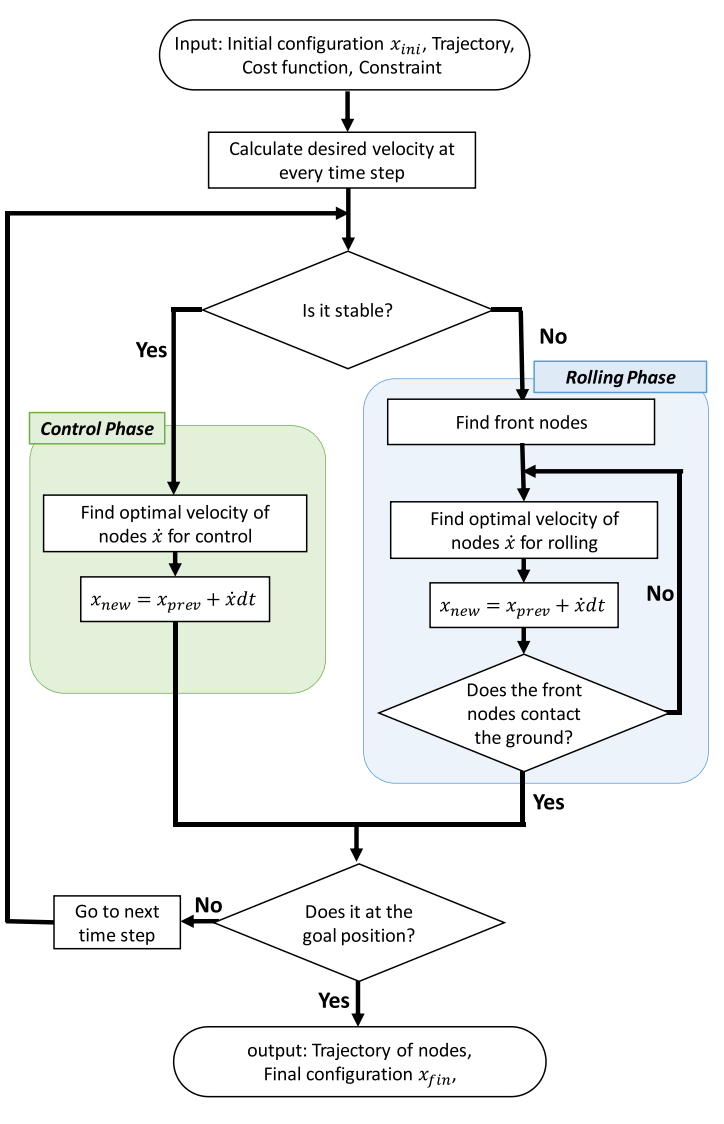
\includegraphics[height=44mm]{elements/[9]-LOCO.png}}
        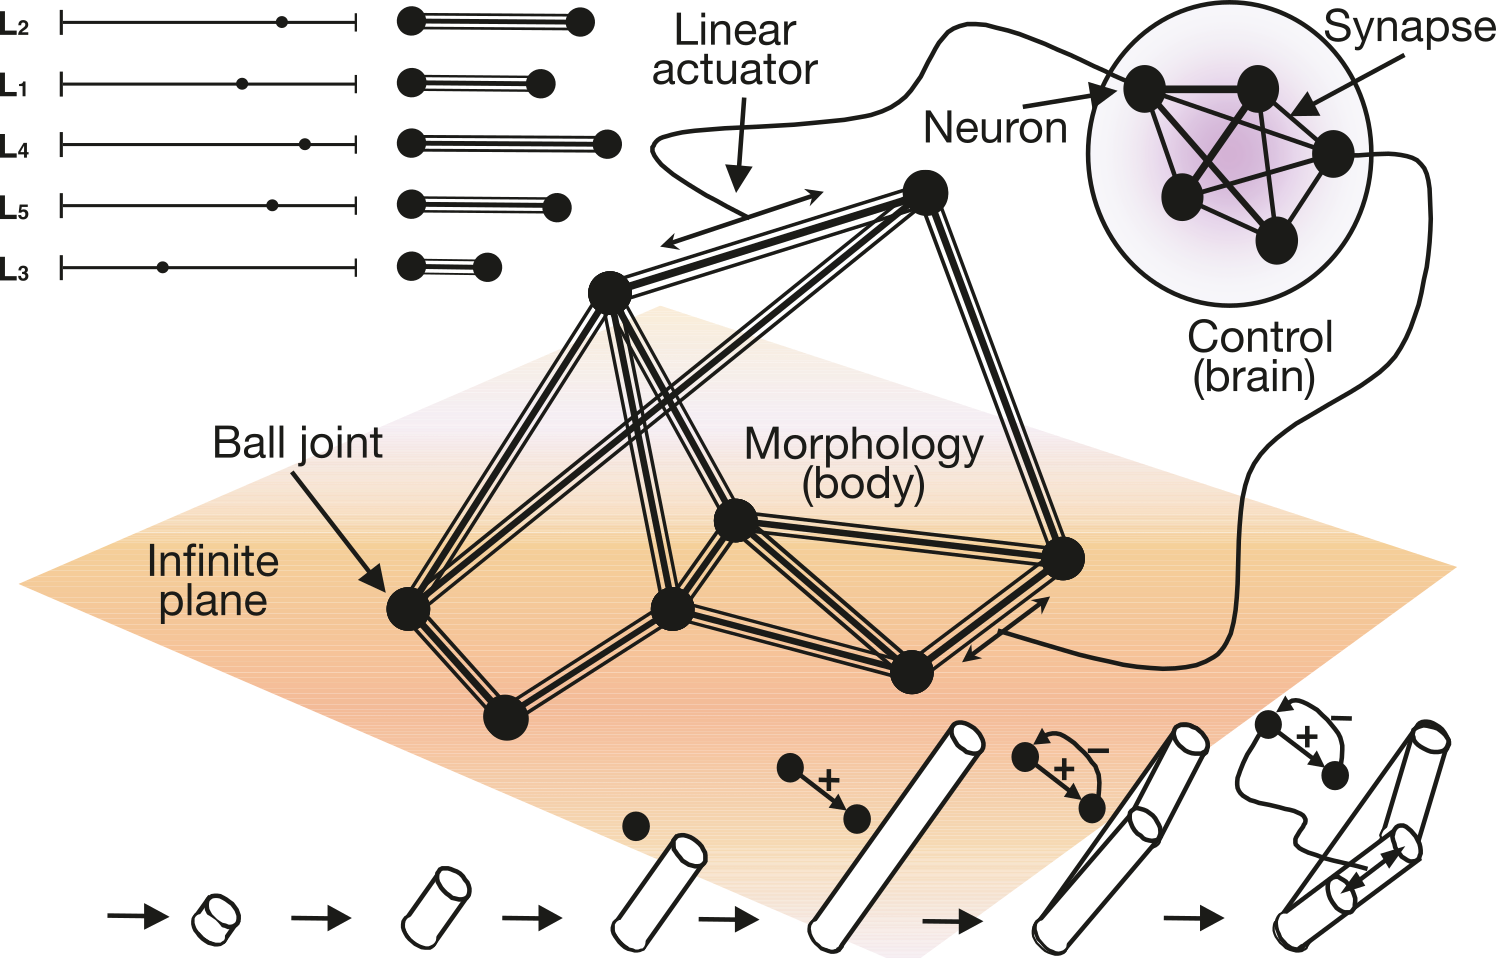
\includegraphics[height=42mm]{elements/[7]-Morphology.png}
        \end{textblock*}

         \uline{\textit{Development of a reinforcement learning based locomotion strategy for truss robots.}}
         This involves coordinating the movement of various parts in a specific sequence, similar to how serpents or mammals move, where intricate coordination is necessary.

        \bigskip
        
        \begin{tikzpicture}
          % \draw [->] (1,1) |-  (2,-3) node[pos=0.25,above,sloped] {Idea Development};
            \draw [->] (1,0) node[yshift=1.5cm,rotate=90] {Idea Development} |-  (1.5,-1.1);
        \end{tikzpicture}

        \begin{textblock*}{60mm}(7mm,-40mm)
        The structure consists of $\mathrm{N}$ linear actuators, each with a single degree of freedom ($\mathrm{DoF}$), interconnected with passive joints.
        
        \begin{enumerate}
            \item \textit{Model-Based/Free RL:} Single topology, baseline for comparison.
            \item \textit{Modular Control Policy RL:} Multiple topology, generalizability.
            \item \textit{Multi-Agent Policy RL:} Each member is an individual agent.
        \end{enumerate}
        
        \end{textblock*}
        
        \begin{textblock*}{5cm}(135mm, -1mm) % {block width} (coords)
        {\tiny \cite{Lipson2000}}
        \end{textblock*}
        \vfill
 
\end{frame}

\section{Literature Review}

\begin{frame}[fragile]{\fontsize{10}{10}\selectfont\textbf{[Non-impact Rolling Locomotion of a Variable Geometry Truss]} \hfill \fontsize{8}{8}\selectfont LITERATURE REVIEW \newline [2019]}
    
        \begin{textblock*}{5cm}(0mm,12mm) % {block width} (coords)
        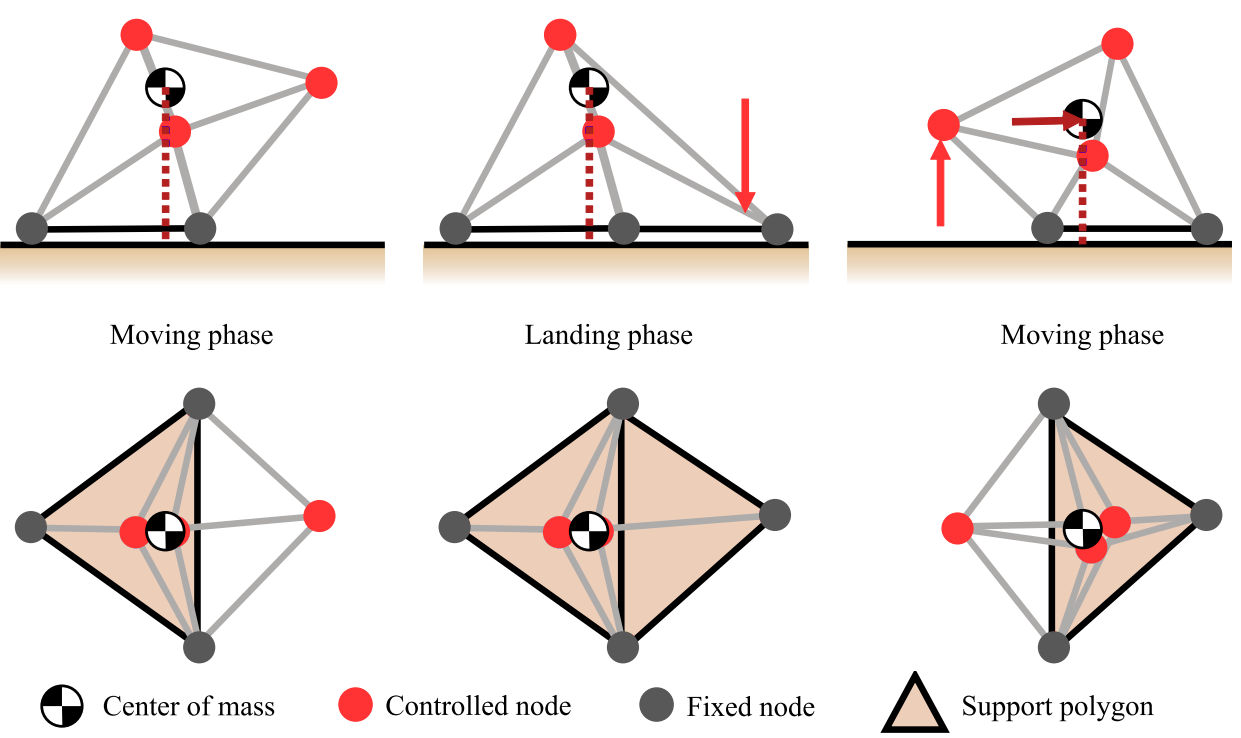
\includegraphics[height=46mm]{elements/[8]-LOCO.png}
        \end{textblock*}

        \begin{textblock*}{5cm}(90mm,-3mm) % {block width} (coords)
        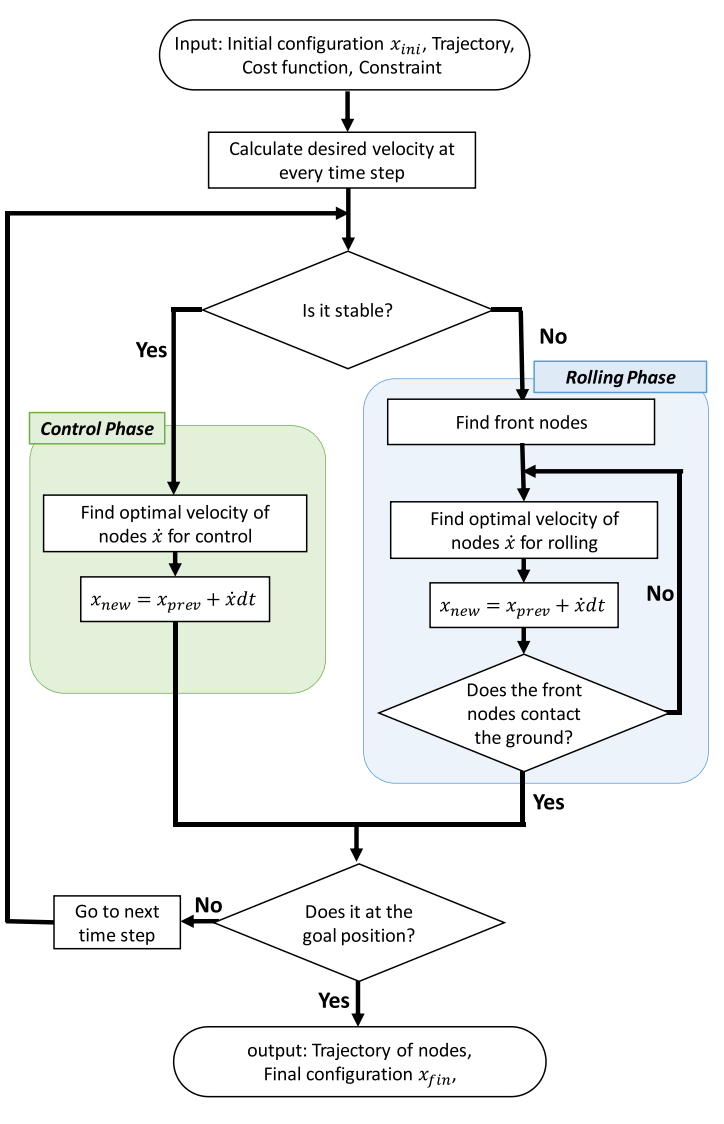
\includegraphics[height=65mm]{elements/[9]-LOCO.png}
        \end{textblock*}

        \begin{textblock*}{87mm}(0mm,-2mm)
        The velocity of nodes is optimized to move the center of mass given the desired velocity. The member velocities are calculated and actuated accordingly.$^{\text{\cite{Usevitch}}}$
        \end{textblock*}

        \begin{textblock*}{5cm}(133mm, 58mm) % {block width} (coords)
        {\tiny \cite{8610002}}
        \end{textblock*}

        \begin{textblock*}{5cm}(75mm, 58mm) % {block width} (coords)
        {\tiny \cite{bb}}
        \end{textblock*}
        
        \vspace{52mm}
\end{frame}

\begin{frame}[fragile]{\fontsize{10}{10}\selectfont\textbf{[Learning Modular Robot Control Policies]} \hfill \fontsize{8}{8}\selectfont LITERATURE REVIEW \newline [2023]}
    
        \begin{textblock*}{5cm}(0mm,17mm) % {block width} (coords)
        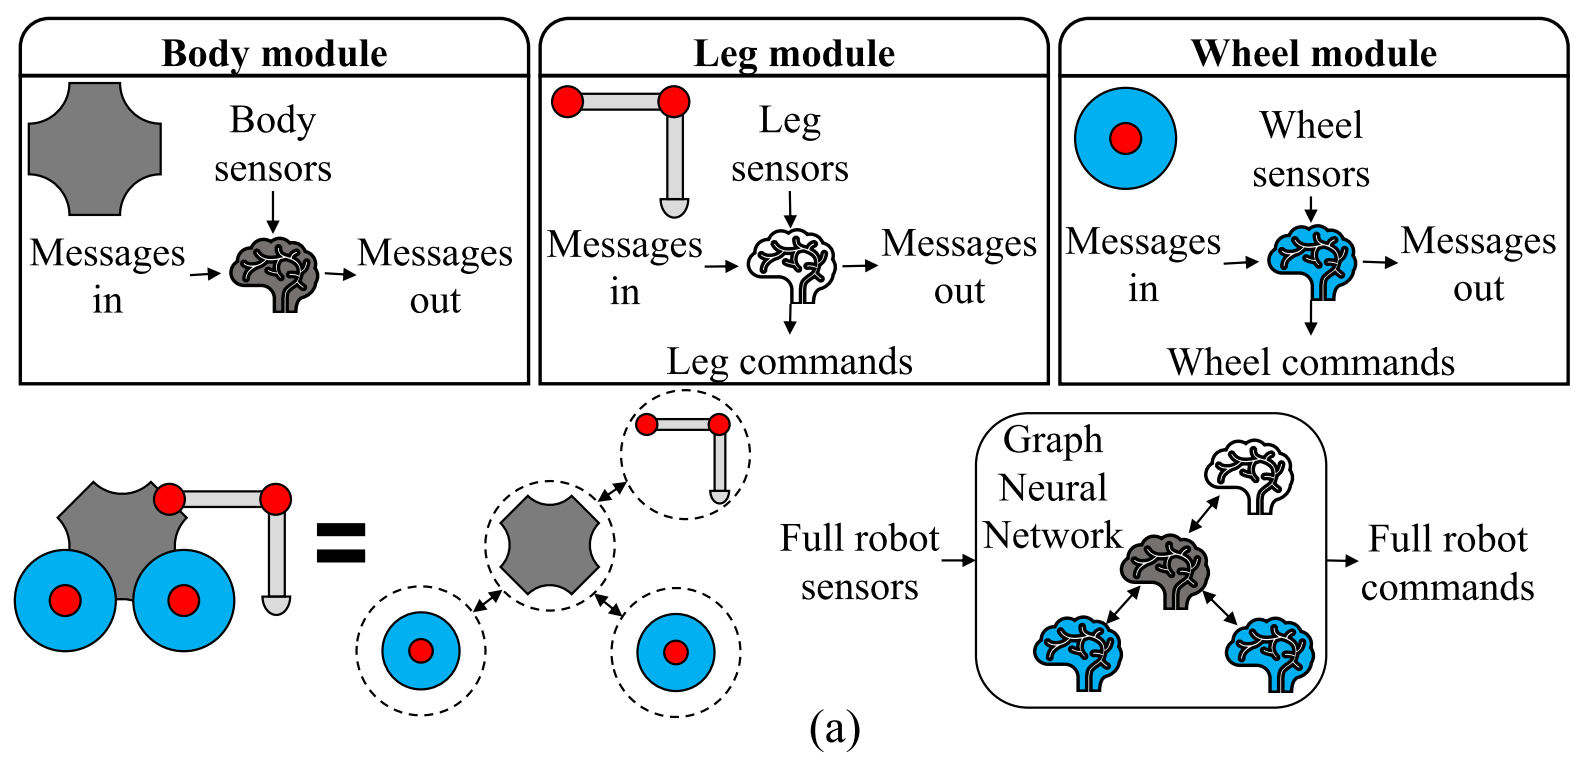
\includegraphics[height=40mm]{elements/[10]-Modular.png}
        \end{textblock*}

        \begin{textblock*}{5cm}(85mm,-3mm) % {block width} (coords)
        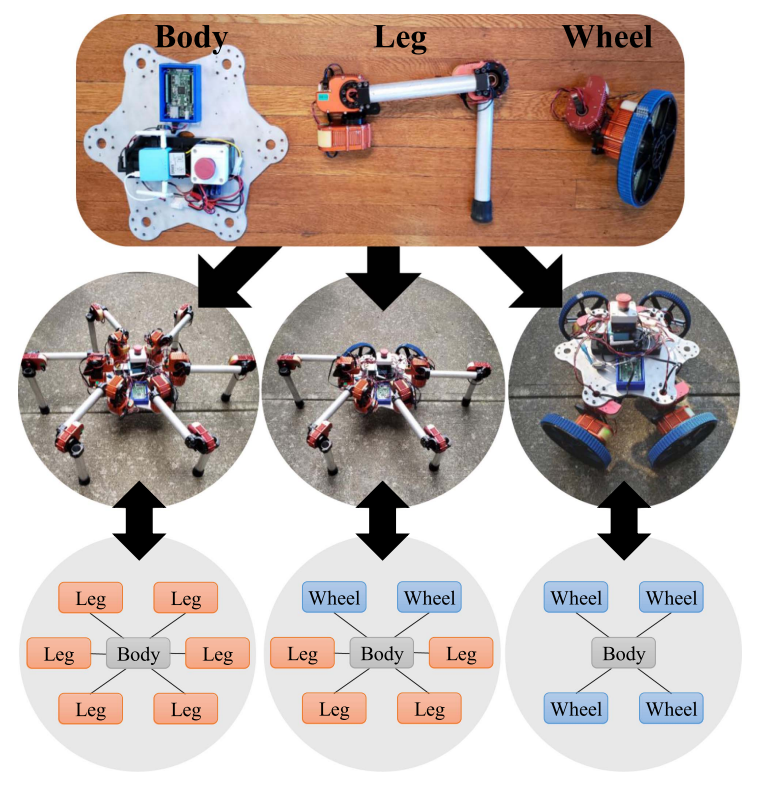
\includegraphics[height=59mm]{elements/[11]-Modular.png}
        \end{textblock*}

        \begin{textblock*}{87mm}(0mm,-2mm)
        Modular robots need specific control policies for each design, which becomes impractical for scalability. A modular policy framework allows for a single training process to adapt to various hardware arrangements and control different designs efficiently.$^{\text{\cite{10167528}}}$
        \end{textblock*}

        \begin{textblock*}{5cm}(133mm, 58mm) % {block width} (coords)
        {\tiny \cite{10167528}}
        \end{textblock*}

        \begin{textblock*}{5cm}(75mm, 58mm) % {block width} (coords)
        {\tiny \cite{10167528}}
        \end{textblock*}
        
        \vspace{52mm}
\end{frame}

\begin{frame}[fragile]{\fontsize{10}{10}\selectfont\textbf{[Distributed Coach-Based RL Controller for Snake Robot Locomotion]} \hfill \fontsize{8}{8}\selectfont LITERATURE \newline [2022]}


        \begin{textblock*}{5cm}(78mm,-11mm) % {block width} (coords)
        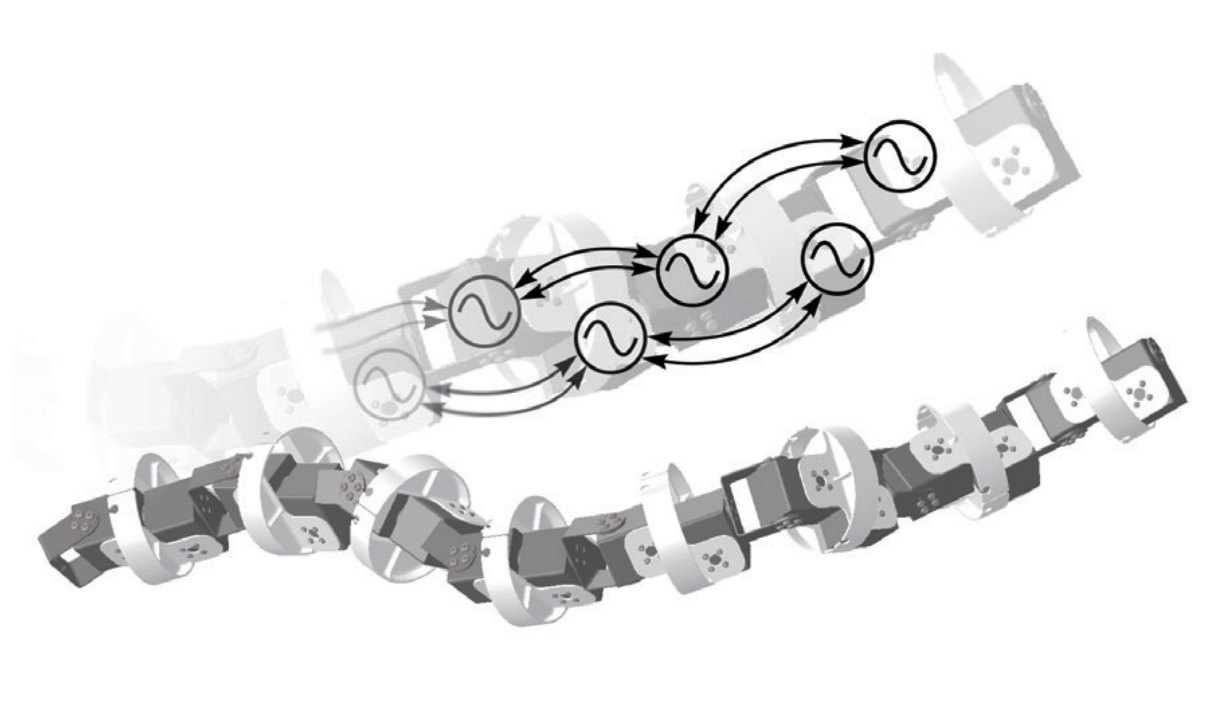
\includegraphics[height=38mm,angle=50,origin=c]{elements/[13]-Snake.png}
        \end{textblock*}
        
        \begin{textblock*}{5cm}(0mm,17mm) % {block width} (coords)
        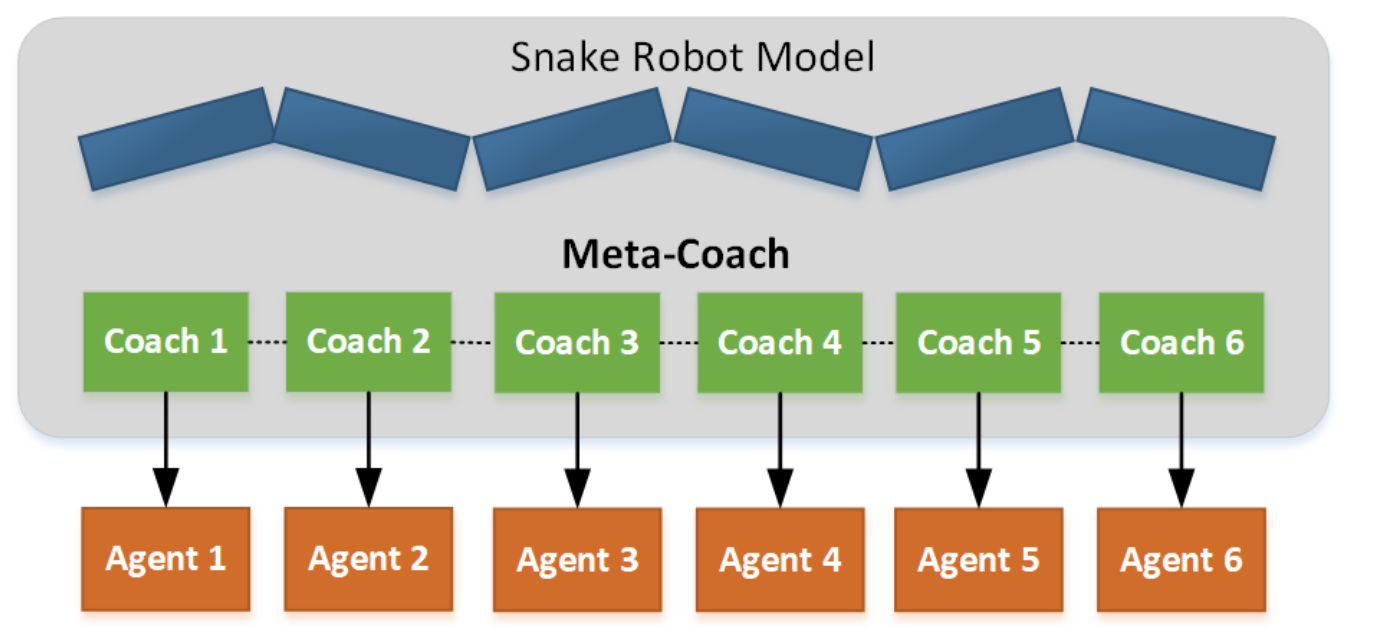
\includegraphics[height=40mm]{elements/[12]-Snake.png}
        \end{textblock*}

        \begin{textblock*}{87mm}(0mm,-2mm)
        Snake robot control with RL is underexplored due to high freedom redundancy. Existing methods use asynchronous joint state representations. A new solution introduces a distributed coach-based learning approach to address these challenges.$^{\text{\cite{9981749}}}$
        \end{textblock*}

        \begin{textblock*}{5cm}(133mm, 58mm) % {block width} (coords)
        {\tiny \cite{9517436}}
        \end{textblock*}

        \begin{textblock*}{5cm}(75mm, 58mm) % {block width} (coords)
        {\tiny \cite{9981749}}
        \end{textblock*}
        
        \vspace{52mm}
\end{frame}

\section{Methodology \& Algorithms}

\begin{frame}[fragile]{\textbf{Developmental Procedure} \hfill \fontsize{8}{8}\selectfont METHODS / ALGORITHMS}
    
        \begin{textblock*}{5cm}(87mm,-15mm) % {block width} (coords)
        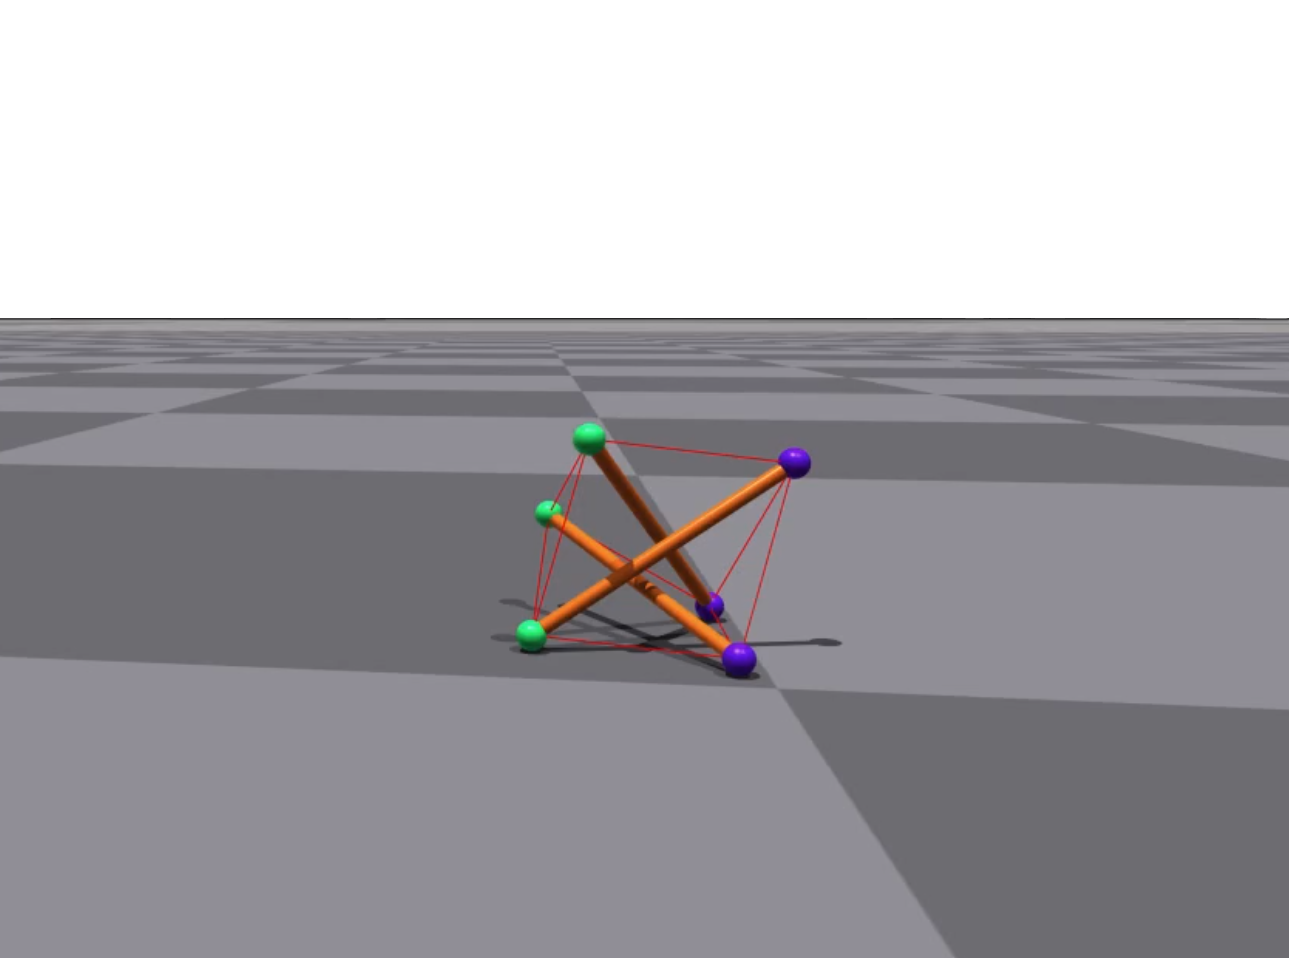
\includegraphics[trim={11cm 3cm 10cm 10cm},clip,height=40mm]{elements/[14]-Tensegrity.png}
        \end{textblock*}

        % https://vimeo.com/70863416

        \begin{textblock*}{138mm}(0mm,-22mm)
         Training simulations will be conducted in NVIDIA$^{\text{®}}$ Isaac Gym, where diverse truss robot models, including the inverse kinematics, will be modeled.
        
        \begin{itemize}
            \item Start with a simple VGT robot, such as a Tetrahedron.
            \item Begin in a uniform flat environment:
            \begin{itemize}
                \item No obstacles (static/dynamic)
                \item No terrain features
            \end{itemize}
            \item Use only proprioceptive sensors and pseudo sensors:
            \begin{itemize}
                \item All measurements are assumed accurate
                \item No point cloud data
                \item No visual feedback
            \end{itemize}
        \end{itemize}

        \bigskip

        \textbf{Algorithms:} Various PPO implementations are available, but they are often targeted for specific applications. A modified PPO implementation is anticipated.$^{\text{\tiny \cite{shi2020circus}}}$

        \end{textblock*}

\end{frame}


\section{Risks \& Limitations}

\begin{frame}[fragile]{\textbf{Assessing the Feasibility} \hfill \fontsize{8}{8}\selectfont RISKS / LIMITATIONS}

        \begin{textblock*}{5cm}(74mm,0mm) % {block width} (coords)
        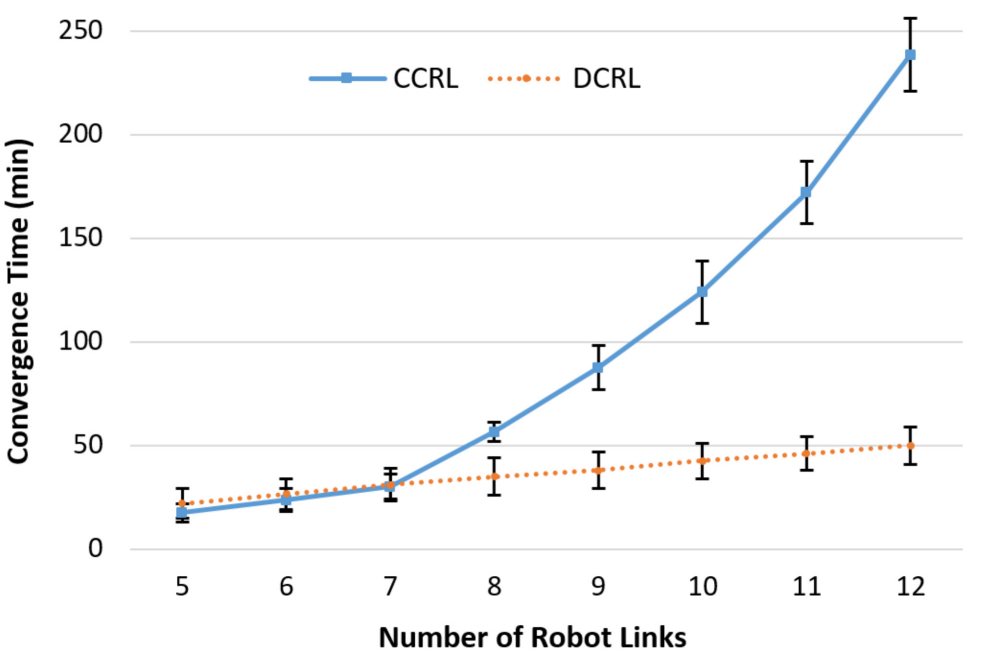
\includegraphics[height=42mm]{elements/[15]-Scaling.png}
        \end{textblock*}

        \begin{textblock*}{138mm}(0mm,-18mm)
        For large-scale robots with numerous linear actuators, convergence times are anticipated to increase rapidly. An octahedral robot, composed of 12 members, essentially mirrors a quadruped robot. Scaling effort necessitates a broader approach. This observation is also mentioned in \cite{9981749}.
        \end{textblock*}

        \begin{textblock*}{110mm}(0mm,-5mm)
        \begin{itemize}
            \item Self collision check required, some truss typologies confine themselves.
            \item Ground contact sensing might be needed.
            \item Alternative simulation environments, 
                \begin{itemize}
                    \item MuJoCo
                    \item RaiSim
                \end{itemize}
            \item Modular control policy approach might \\
            increase the input size even further.
            \item Proper reward mechanism design leads to \\
            more advanced locomotion.
        \end{itemize}
        \end{textblock*}

        \begin{textblock*}{5cm}(135.5mm, 39mm) % {block width} (coords)
        {\tiny \cite{9981749}}
        \end{textblock*}

        \vspace{10mm}

\end{frame}

\section{Contributions \& Future Work}

\begin{frame}[fragile]{\textbf{Contributions \& Future Works}}

    % \begin{textblock*}{5cm}(9mm,12.7mm) % {block width} (coords)
    % 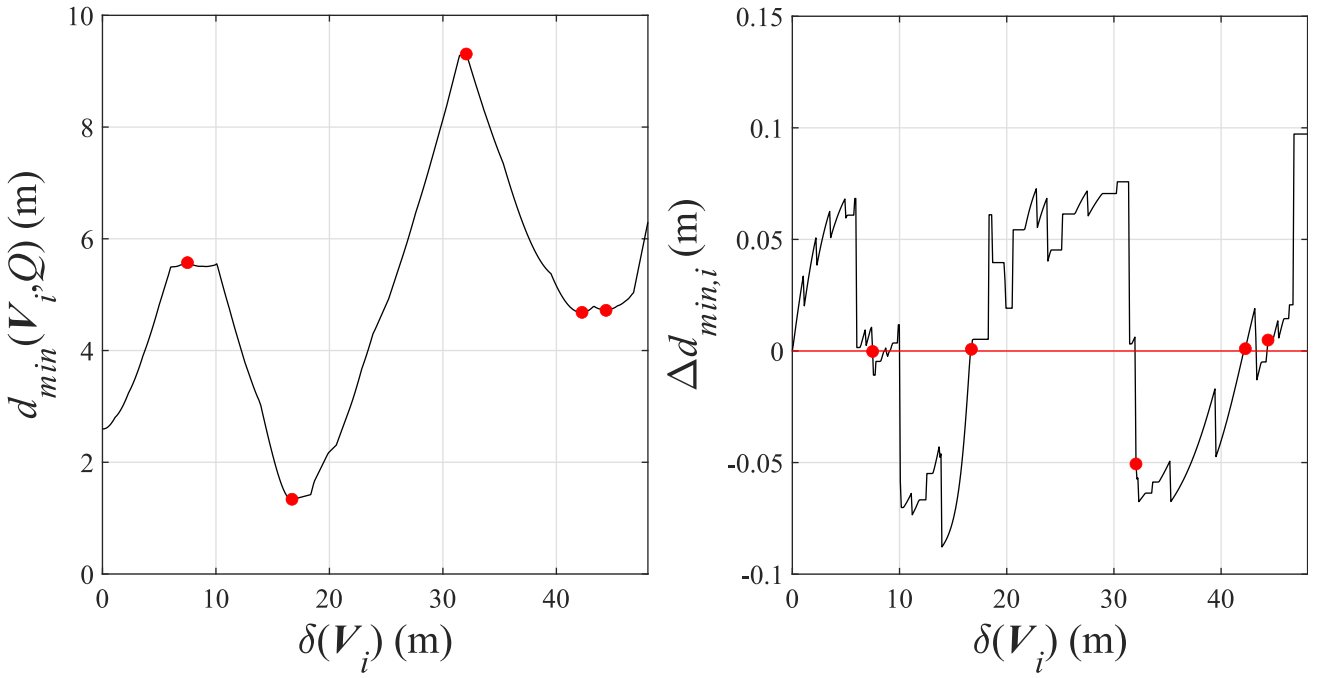
\includegraphics[height=30mm]{elements/[21]-PRT-V.png}
    % \end{textblock*}

    \begin{textblock*}{5cm}(46mm,8mm) % {block width} (coords)
    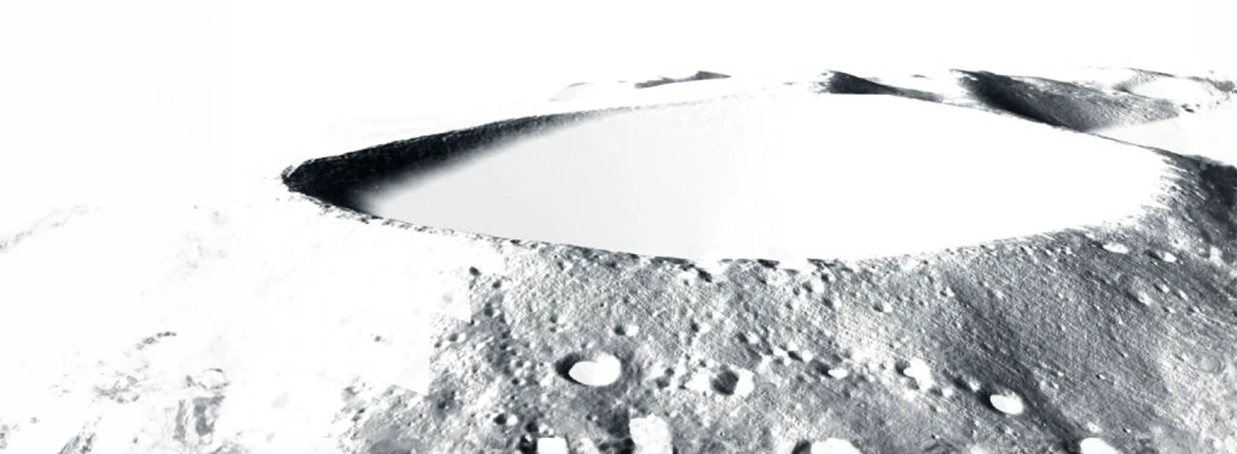
\includegraphics[height=34mm]{elements/[16]-Future.png}
    \end{textblock*}

    \begin{textblock*}{138mm}(0mm,-20mm)

    \vspace{2mm}

    \begin{itemize}
        \item Assess the applicability and scalability of reinforcement learning methods across truss robots of different sizes and topologies.
        \item Evaluate and document the generalizability of the pipeline for robots with various \\ topologies.
        \item Adapt locomotion and path planning strategies to navigate \\ irregular, non-planar terrains.
        \item Tensegrity robot locomotion is intended.
    \end{itemize}
    \end{textblock*}

    \vspace{10mm}

\end{frame}

\begin{frame}[allowframebreaks]{Bibliography}
    \setbeamercolor{bibliography}{fg=black}
    \bibliographystyle{ieeetr}
    \bibliography{refs.bib}
\end{frame}

\begin{closingframe}
    \smallskip
    {\Large Thank you for listening}
    % \begin{textblock*}{5cm}(50mm,-5mm) % {block width} (coords)
    % 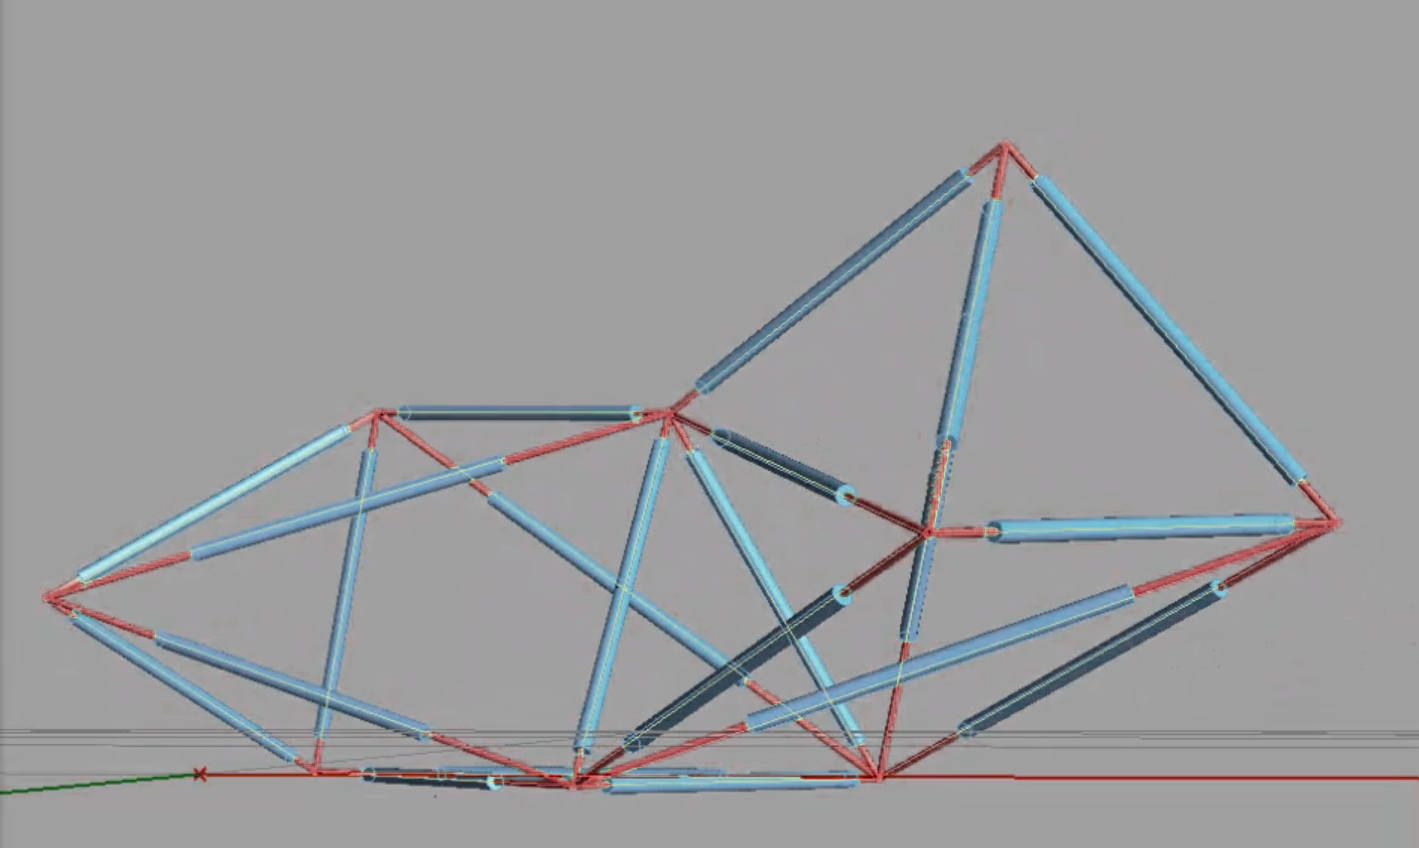
\includegraphics[height=50mm]{elements/[25]-Future.png}
    % \end{textblock*}
    \medskip
    \vspace{10mm}
\end{closingframe}

\end{document}